% $Id$

%==============================================================================
\section{Remote Component Structure}
%==============================================================================

While we have implemented a local version of CORBA Components, 
the LwCCM specification defines remote components only.
Remote components are built up from CORBA objects that implement defined
IDL interfaces.
Because of the specified mapping from IDL3 to IDL2, the generated IDL2 files 
can be processed by every existing IDL compiler. In addition to CORBA stubs
and skeletons, remote component logic as well as CORBA component containers
must be implemented too. 
To be compliant to the LwCCM specification, we have developed a way to
adapt local components into remote LwCCM components - the 
{\bf Local Component Adapter Concept} (LCAC).

LCAC allows to add remote communication
for each port transparently for business logic.
Fig.~\ref{LcacOverview} shows how a given local component implementation
can be extended to a remote LwCCM component.

\begin{figure}[htbp]
    \begin{center}
    \includegraphics [width=5.5cm,angle=0] {figures/LocalAdapterConcept.eps}
    \caption{A local component can be embedded in a remote component logic
    that will be managed by a remote component container.}
    \label{LcacOverview}            
    \end{center}
\end{figure}

\noindent
The point is that we can use local components without changing them.
Thus, for a remote accessible component that provides at least one remote 
port, some additional code will be involved.

\begin{description}
\item [Remote component logic.]
A glue code layer is responsible for embedding a local component into a 
remote CORBA component. 
This remote component logic hosts a local component.
That means, its local component logic and business logic.  
Such a structure ensures that local ports can be used side by side to remote
ports.

\item [Adapter set.]
For a given IDL interface that defines a component port's syntax, a local and 
a remote implementation is generated. 
Using a set of adapter classes, these two worlds can fit together transparently.
In addition to component ports, adapters must be provided for component homes
as well as the component's equivalent interface.

\item [Remote component container.]
For each remote component type, a generic component container is used to
manage CORBA component instances.
In contrast to a local component container that can have a simple structure, a
remote container is also responsible for sophisticated {\it Quality of Service} 
(QoS) tasks.

\item [Remote container runtime environment.]
With increasing QoS functionality, the requirements to a remote container
runtime environment are growing too.
Besides an {\it Object Request Broker} (ORB), that handles CORBA requests,
libraries for multi--threading and process management implementation must 
be available.  
\end{description}

\noindent
This adapter concept is a powerful tool especially in heterogeneous 
environments. Besides the choice between local and remote connections, 
a deployment process can also decide to use different middleware technologies.


The fact that a local component is wrapped by a remote component becomes 
obvious from Fig.~\ref{StructureOfRemoteComponents}. All classes of a local
component remain unchanged, while some new ``remote'' classes have been added.

\begin{figure}[htbp]
    \begin{center}
    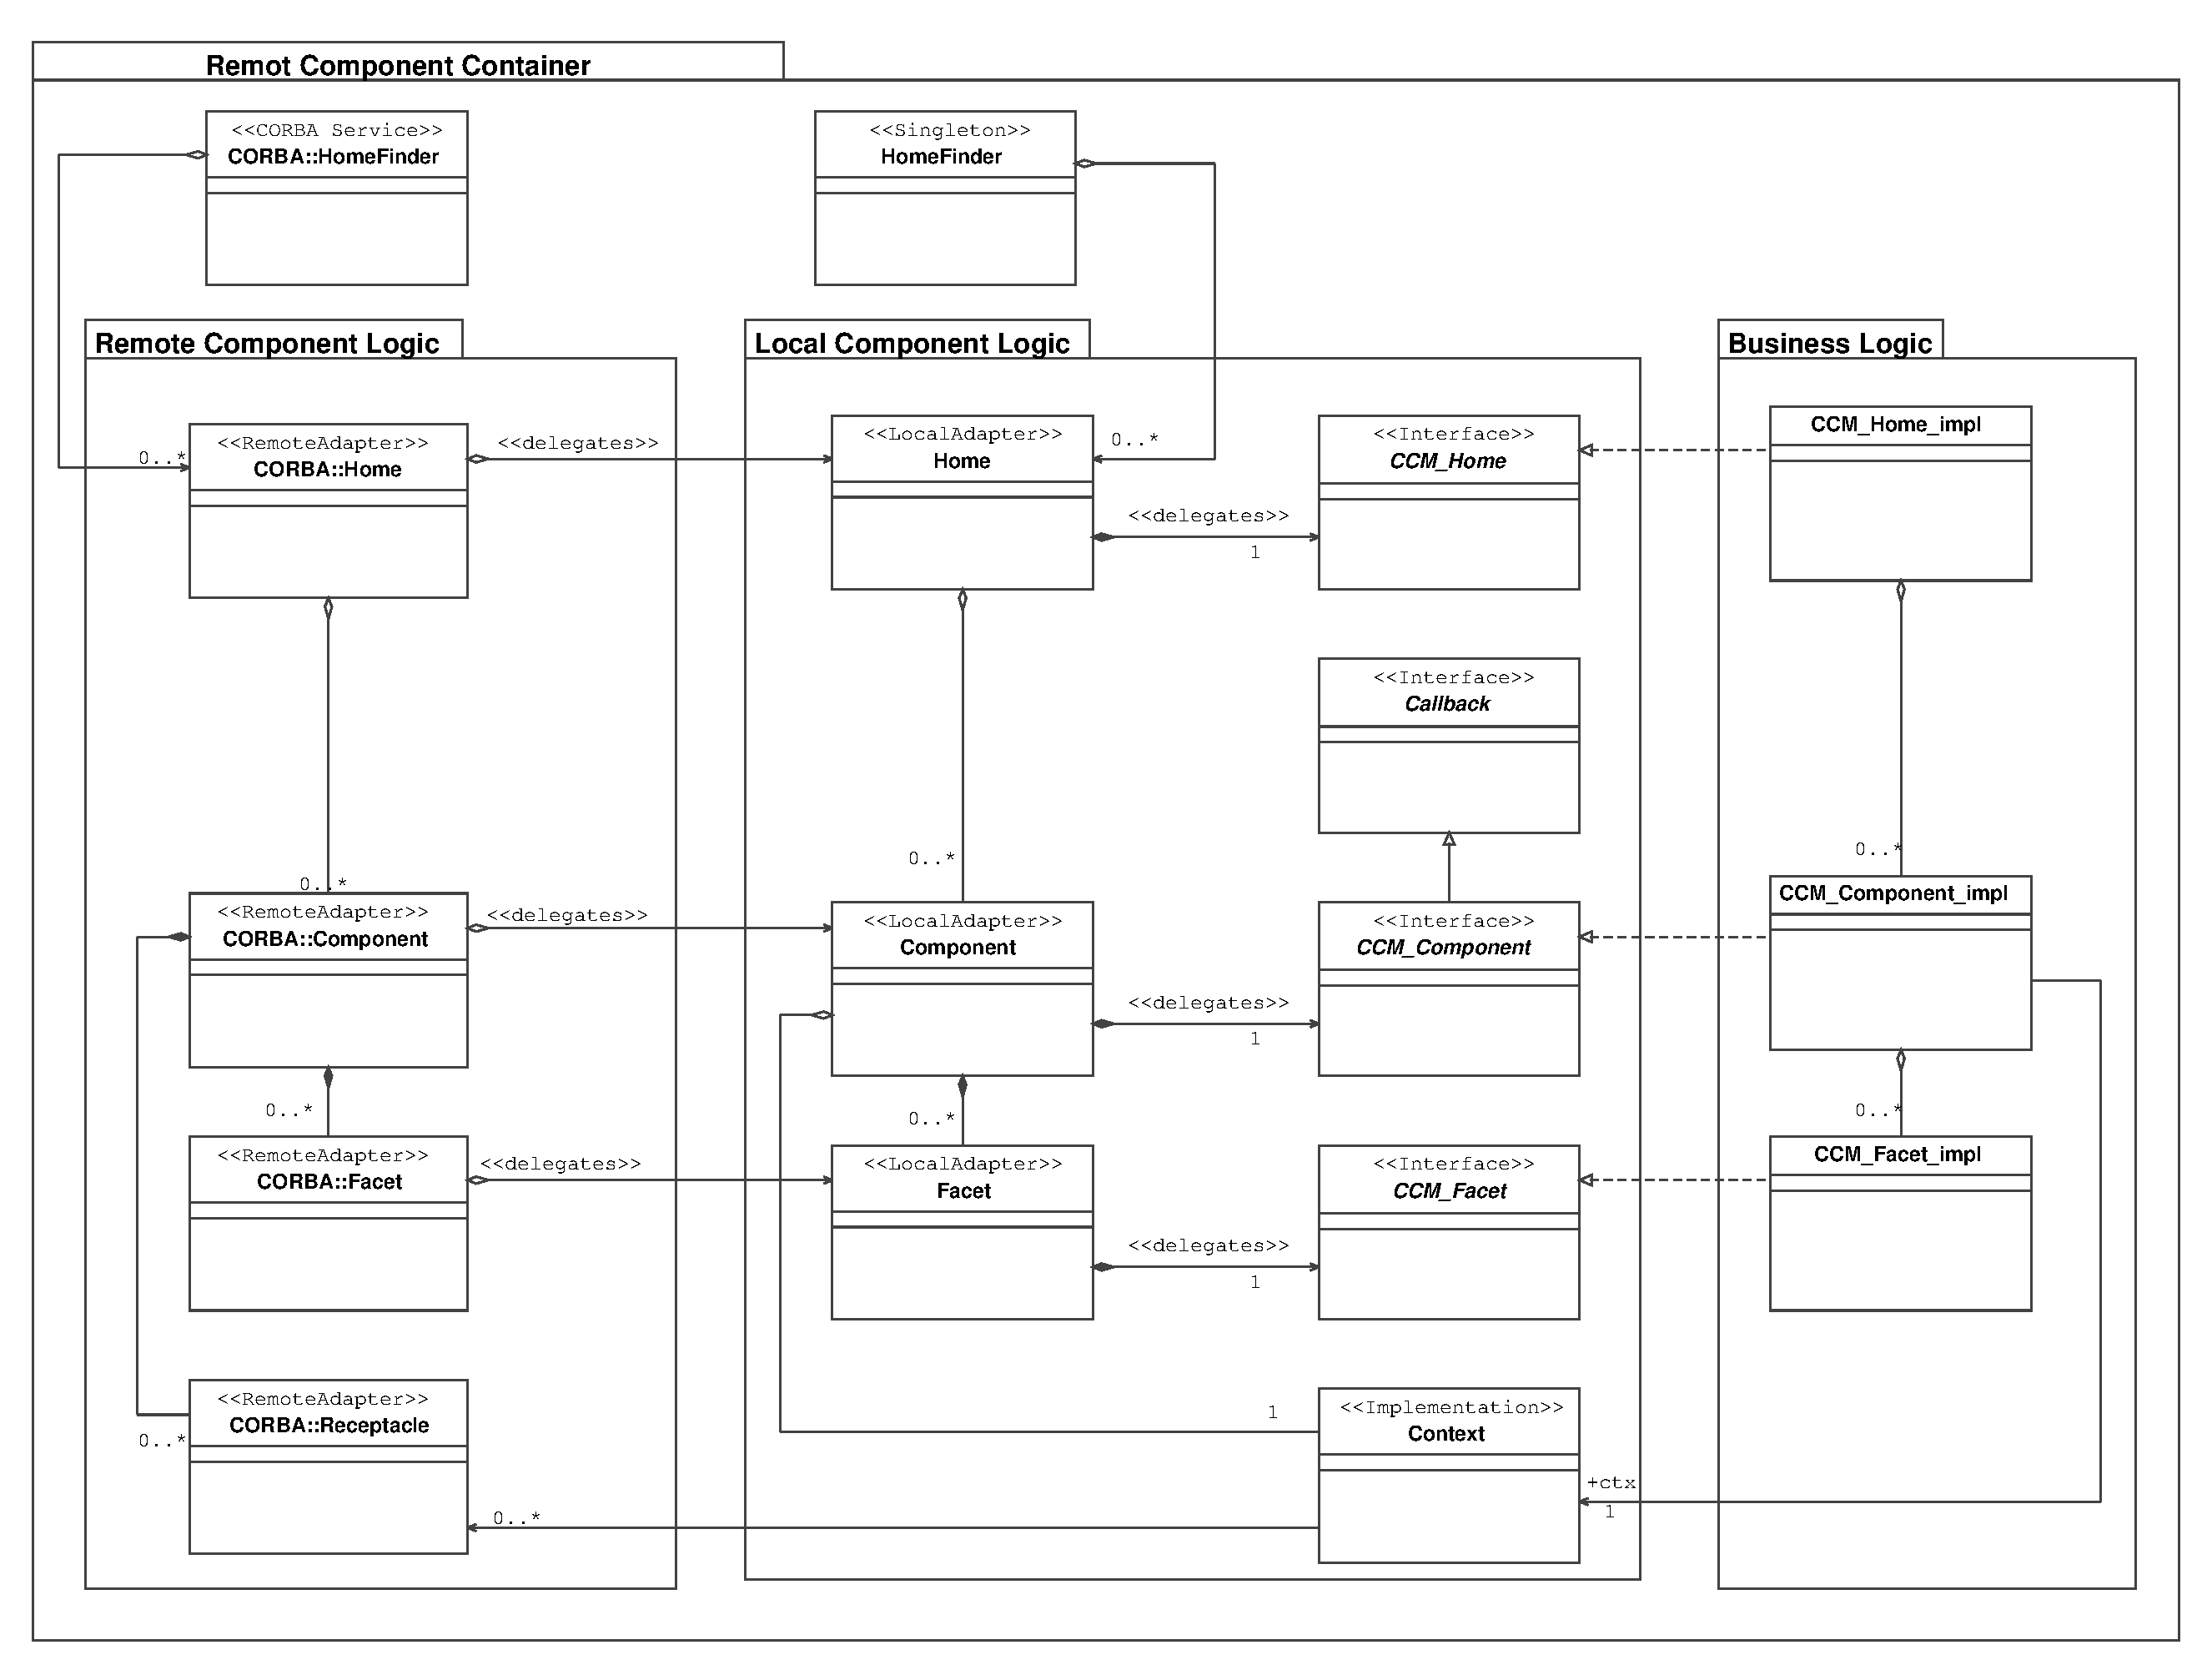
\includegraphics [width=15cm,angle=0] 
		     {uml/StructureOfRemoteComponents.eps}
    \caption{Simplified structure of a remote component implementation,
    showing the relationship between corresponding local and remote components.}
    \label{StructureOfRemoteComponents}            
    \end{center}
\end{figure}

\noindent
The remote structure is very similar to a local component's structure 
(Fig.~\ref{StructureOfLocalComponents}), thus, we can compare interactions
between a local and a remote component with interactions between business logic
and local component logic:

\begin{description}
\item [Calling component methods.]
A remote client calls methods on a remote adapter that delegates this
calls to a local component which uses a local adapter to delegate these calls
to business logic.
In each adapter, pre- and a post-invoke processing can take place 
(Fig.~\ref{RemoteComponentCall}).
\begin{figure}[htbp]
    \begin{center}
    \includegraphics [width=9cm,angle=0] 
		     {figures/RemoteComponentCall.eps}
    \caption{A remote call of a component's method is delegated twice
    allowing pre- and post-invoke processing.}
    \label{RemoteComponentCall}            
    \end{center}
\end{figure}

These two indirection layers allow non--functional extensions to 
components without changes in business logic. 
This separation of concerns is a cornerstone in component
based development.

\item [Invoking callback methods.]
Callback methods implemented by business logic can be
triggered either from local or remote component logic and their corresponding
container implementations to control a component's life cycle.

\item [Using context methods.]
Component business logic uses the {\tt Context} object to access container
functionality as well as component receptacles.
In the case of remote components, receptacles can be either local or remote
ports. Both kinds of receptacles can be accessed via local context
object methods. While local receptacles are connected directly to local facets,
remote receptacles are intercepted by a receptacle adapter.
\end{description}

\noindent
Based on LCAC, an existing LwCCM container implementation could be used to host 
local components, thus, we could combine an existing CORBA application server 
with the presented extensions in the context of local components. 



\newpage
%==============================================================================
\section{Car rental example}
%==============================================================================

We reuse our well known {\tt CarRental} component
to show how a local component can be extended to a CORBA component.
The local {\tt CarRental} component is organized in the following file 
structure:

\begin{small}
\begin{verbatim}
   CarRental
   |-- idl3
   |   |-- component
   |   |   `-- BigBusiness
   |   `-- interface
   |       `-- BigBusiness
   `-- server
       |-- component
       |   `-- CarRental
       |       |-- CCM_Local_BigBusiness_CCM_Session_CarRental
       |       |-- CCM_Local_BigBusiness_CCM_Session_CarRental_share
       |       `-- impl
       `-- interface
           `-- CCM_Local_BigBusiness
\end{verbatim}
\end{small}


%------------------------------------------------------------------------------
\subsubsection{Generate CORBA component adapters}
%------------------------------------------------------------------------------

For a remote CORBA component all IDL3 files must be mapped to equivalent
IDL2 files, as defined in the CCM specification \cite{CCMSpecification}.
Using the CCM Tools, this mapping can be done with a single call: 
\begin{small}
\begin{verbatim}
> ccmtools idl2 -o server/CORBA_Stubs \ 
                -Iserver/idl3/interface \ 
                -Iserver/idl3/component \
                server/idl3/interface/BigBusiness/*.idl \
                server/idl3/component/BigBusiness/CarRental.idl \
                server/idl3/component/BigBusiness/CarRentalHome.idl
\end{verbatim}
\end{small}

The result of this IDL3 to IDL2 mapping is a {\tt CORBA\_Stubs} subdirectory,
where all IDL2 files are stored. Additionally, the generated 
{\tt CORBA\_Stubs/Makefile}
triggers Mico's IDL compiler to create C++ stub and skeleton files during
the {\tt Confix} build process.

\begin{small}
\begin{verbatim}
server/
|-- CORBA_Stubs
|   |-- BigBusiness_CarRental.idl
|   |-- BigBusiness_CarRentalHome.idl
|   |-- BigBusiness_CreateCustomerException.idl
|   |-- BigBusiness_Customer.idl
|   |-- BigBusiness_CustomerBusiness.idl
|   |-- BigBusiness_CustomerList.idl
|   |-- BigBusiness_CustomerMaintenance.idl
|   |-- BigBusiness_NoCustomerException.idl
|   |-- BigBusiness_RemoveCustomerException.idl
|   |-- Makefile
|   |-- Makefile.py
|   `-- build.xml
\end{verbatim}
\end{small}

Besides the CORBA stubs and skeletons, a set of adapters is needed to
convert between CORBA objects and local component classes.
These component adapters are generated with the following call:
\begin{small}
\begin{verbatim}
> ccmtools c++remote -o server/component/CarRental \
                     -Iserver/idl3/interface \
                     -Iserver/idl3/component \
                     server/idl3/interface/BigBusiness/*.idl \
                     server/idl3/component/BigBusiness/CarRental.idl \
                     server/idl3/component/BigBusiness/CarRentalHome.idl
\end{verbatim}
\end{small}

This additional component logic is stored within the {\tt CarRental}
component directory (see {\tt CCM\_Remote\_*} and {\tt CORBA\_Converter}
subdirectories).
Remember, the LCAC allows to extend a local component to a CORBA component
without business logic changes. 
\begin{small}
\begin{verbatim}
server/
|-- component
|   |-- CarRental
|   |   |-- CCM_Local_BigBusiness_CCM_Session_CarRental
|   |   |-- CCM_Local_BigBusiness_CCM_Session_CarRental_share
|   |   |-- CCM_Remote_BigBusiness_CCM_Session_CarRental
|   |   |-- CORBA_Converter
|   |   |-- Makefile.py
|   |   `-- impl
|   `-- Makefile.py
\end{verbatim}
\end{small}


%------------------------------------------------------------------------------
\subsubsection{Install the remote {\tt CarRental} component}
%------------------------------------------------------------------------------
Finally, we can run {\tt Confix} to build and install this remote component:
\begin{small}
\begin{verbatim}
> confix.py --packageroot=`pwd`/server --bootstrap --configure 
            --make --targets=install
\end{verbatim}
\end{small}



%------------------------------------------------------------------------------
\subsubsection{Implement a CORBA component server}
%------------------------------------------------------------------------------

A remote component must be started in its own process to handle CORBA calls
from clients or other remote components.
The {\tt server.cc} code, stored in the {\tt CORBA\_Server} subdirectory, 
shows a minimal implementation of such a CORBA component server.

\begin{small}
\begin{verbatim}
server/
|-- CORBA_Server
|   |-- Makefile.py
|   `-- server.cc
|-- CORBA_Stubs
|-- component
|-- idl3
`-- interface
\end{verbatim}
\end{small}

After setting up the ORB, both local and remote component are deployed.
Deployment of a remote component implies the registration to a CORBA NameService.
Finally, the ORB is turned to its run mode to handle incoming CORBA requests.

\begin{small}
\begin{verbatim}
#include <cstdlib> 
#include <iostream>
#include <string>
#include <WX/Utils/debug.h>
#include <CCM/CCMContainer.h>

#include <CORBA.h>
#include <coss/CosNaming.h>

#include <CCM_Remote/BigBusiness/CCM_Session_CarRental/CarRentalHome_remote.h>
#include <BigBusiness_CarRental.h>

using namespace std;
using namespace WX::Utils;

int main (int argc, char *argv[])
{
    // Initialize ORB 
    CORBA::ORB_var orb = CORBA::ORB_init(argc, argv);

    // Register all value type factories with the ORB  
    CCM::register_all_factories (orb);

    // Deploy local and remote component homes	
    int error = 0;
    error += 
        deploy_CCM_Local_BigBusiness_CarRentalHome("CarRentalHome");
    error += 
        deploy_CCM_Remote_BigBusiness_CarRentalHome(orb, "CarRentalHome:1.0");
    if(!error) {
        cout << "CarRentalHome server is running..." << endl;
    }
    else {
        cerr << "ERROR: Can't deploy components!" << endl;
        return -1;
    }

    // Start ORB
    orb->run();
}
\end{verbatim}
\end{small}

Before we can build the {\tt CarRental} server with a well known Confix call, 
we have to create an empty {\tt Makefile.py} file, forcing Confix to build 
this new directory.

\begin{small}
\begin{verbatim}
> touch server/CORBA_Server/Makefile.py
> confix.py --packageroot=`pwd`/server --bootstrap --configure 
            --make --targets=install
\end{verbatim}
\end{small}

A distributed CCM application uses CORBA's NameService to store component
home instances and their names. Mico comes with such a service called {\tt nsd}.
We start this service at port 5050.
\begin{small}
\begin{verbatim}
> nsd -ORBIIOPAddr inet:localhost:5050 -ORBIIOPVersion 1.2
\end{verbatim}
\end{small}

Now, we can run our {\tt CarRental} server which has been installed by Confix to
{\tt \$CCM\_INSTALL/bin}.
\begin{small}
\begin{verbatim}
> $CCM_INSTALL/bin/CarRental_CORBA_Server_server \
      -ORBInitRef NameService=corbaloc:iiop:1.2@localhost:5050/NameService
\end{verbatim}
\end{small}
%$

OK, our first CORBA component server is running - let's try to access it from
a remote client.


\newpage
%------------------------------------------------------------------------------
\subsubsection{Implement a C++ CORBA component client}
%------------------------------------------------------------------------------

CORBA components can be connected to each other to build component assemblies.
In this case, where one component is the client of another component, the
client does not care about the CORBA programming model.
On the other side, when we use a regular CORBA client to access a remote
component, we have to worry about this C++/CORBA stuff.

The following {\tt client.cc} code is stored in a new directory:
\begin{small}
\begin{verbatim}
CarRental
|-- CORBA_Client/
|   |-- Makefile.py
|   `-- client.cc
`-- server
\end{verbatim}
\end{small}


\begin{small}
\begin{verbatim}
#include <CORBA.h>
#include <coss/CosNaming.h>

#include <CCM/CCMContainer.h>

#include <CCM_Remote/BigBusiness/CCM_Session_CarRental/CarRentalHome_remote.h>
#include <BigBusiness_CarRental.h>

using namespace std;
using namespace WX::Utils;

int main (int argc, char *argv[])
{
  try {
    // Init ORB and CORBA NameService
    CORBA::ORB_var orb = CORBA::ORB_init(argc, argv);
    CORBA::Object_var obj = 
      orb->resolve_initial_references("NameService");
    CosNaming::NamingContextExt_var nc =
      CosNaming::NamingContextExt::_narrow(obj);
    
    // Component instantiation
    obj = nc->resolve_str("CarRentalHome:1.0");
    assert (!CORBA::is_nil (obj));
    ::BigBusiness::CarRentalHome_var myCarRentalHome = 
        ::BigBusiness::CarRentalHome::_narrow (obj);

    ::BigBusiness::CarRental_var myCarRental = 
        myCarRentalHome->create();
    
    ::BigBusiness::CustomerMaintenance_var maintenance = 
        myCarRental->provide_maintenance();
    
    ::BigBusiness::CustomerBusiness_var business = 
        myCarRental->provide_business();
    
    myCarRental->configuration_complete();
    
    
    // Use component instance
    {
      business->dollars_per_mile(5.5);
      CORBA::Long id = 1;
      ::BigBusiness::Customer person;
      person.id = id;
      person.first_name = "Franz";
      person.last_name = "Kafka";
      maintenance->createCustomer(person);
    
      business->resetCustomerMiles(id);
      business->addCustomerMiles(id, 120.0);
    }
    {
      CORBA::Long id = 1;
      ::BigBusiness::Customer_var person = 
           maintenance->retrieveCustomer(id);
      double dollars = business->getCustomerDollars(id); 

      cout << " Customer: " << person->first_name << " " 
           << person->last_name << endl;
      cout << " Miles : " <<  person->mileage << endl;
      cout << " To pay: " << dollars << " Dollars" << endl;
    }

    // Destroy component instance
    myCarRental->remove();
  }
  catch(...) {
    cout << "Client: there is something wrong!" << endl;
    return -1;
  }
}
\end{verbatim}
\end{small}

In the majority of cases, a CORBA component client can be structured in:
\begin{itemize}
\item Initialize the CORBA ORB and the CORBA NameService.

\item Find a component home object, create a component instance and retrieve 
some facet references. Don't forget to finish this instantiation phase with a
{\tt configuration\_complete()} call.

\item Use the component instance and their facets to call some business
logic.

\item Destroy the component instance to free server resources.
\end{itemize} 

That's it, we can build this simple client and run it against our CORBA
component server.

Once again, we define a {\tt Makefile.py} that defines the name and version
of our package and run Confix to build and install this application.
\begin{small}
\begin{verbatim}
> cat CORBA_Client/Makefile.py

PACKAGE_NAME('CorbaClient')
PACKAGE_VERSION('1.0.0')
\end{verbatim}
\end{small}

\begin{small}
\begin{verbatim}
> confix.py --packageroot=`pwd`/CORBA_Client --bootstrap --configure 
            --make --targets=install
\end{verbatim}
\end{small}

To start the client we have to pass some CORBA parameters which define 
the NameService's location:

\begin{small}
\begin{verbatim}
> $CCM_INSTALL/bin/CorbaClient_client \
      -ORBInitRef NameService=corbaloc:iiop:1.2@localhost:5050/NameService
\end{verbatim}
\end{small}
% $

This example can also be tested in a distributed environment - the only thing
you have to ensure is that the right NameService location is passed to both
server and client.


%------------------------------------------------------------------------------
%\subsubsection{Implement a Java CORBA component client}
%------------------------------------------------------------------------------
